\documentclass{article}
\usepackage[utf8]{inputenc}

\usepackage{amsmath}

\usepackage{graphicx}
\graphicspath{{out/}}

\usepackage{float}

\usepackage{chemarr}

\title{Parameter space exploration in the context of a dynamic chemical system}
\author{John Mason}
\date{October 2018}

\begin{document}

\maketitle

This is minimal example of where my `parsimonious' perturbation approach, developed extensively in my paper, is useful.

\section{Motivation}

Optimization, particularly for multimodal optimizaiton problems, is hard.  Most modern advances in optimization don't apply to the sorts of problems we encounter in biological parameter estimation as 1) we lack dense, regular, replicate observation data, and 2) the structures of biological systems tend to be sparse and irregular.  In other words, we need all the help we can get.

In this small study, I compare four different approaches for exploring the parameter space in the context of estimating the parameters of a system of chemical reactions, with terms penalizing for undesirable behaviors as well as poor fit to expected parameter values.

The first two approaches are characteristic of uninformed parameter space exploration.  These correspond to two extreme strategies; either perturbing individual parameters one at a time, or perturbing all of the parameters in a random direction.  Both of these strategies tend to become trapped in unfavorable regions of the objective space.

The second pair of strategies are related to my recently published `parsimonious' perturbation approach.  The first is a `proto'-parsimonious approach -- very much the logical precursor to the true parsimonious approach, which, unlike the other three strategies, is capable of solving this problem reliably.

\section{Model system}

The model system here is a simple, linear chemical reaction pathway, comprising four chemical species (1, 2, 3, and 4), and three reactions (A, B, and C), ala

\begin{align}
c_1 \xrightleftharpoons{k_A} c_2 \xrightleftharpoons{k_B} c_3 \xrightleftharpoons{k_C} c_4
\end{align}

Mathematically,

\begin{align}
	v_A &= k_A \left(c_2 - c_1\right)
\\	v_B &= k_B \left(c_3 - c_2\right)
\\	v_C &= k_C \left(c_4 - c_3\right)
\end{align}

and

\begin{align}
	\dot{c}_2 &= v_B - v_A
	\\ \dot{c}_3 &= v_C - v_B
\end{align}

Chemical species 1 and 4 are not considered dynamically as they are assumed to be outside the system.

\section{Optimization objective}

The goal is simultaneously minimize four terms:

\begin{enumerate}
	\item The absolute deviation from steady-state, expressed as the sum of the squares of the \(\dot{c}_i\) terms.
	\item The relative deviation from steady-state, expressed as the sum of the squares of the \(\dot{c}_i/c_i\) terms.
	\item The square deviation of \(v_C\) from a target flux of 1.
	\item The absolute deviation of \(\log_{10} c_1\) from \(\log_{10} 1 = 0\)
\end{enumerate}

The four terms summed together, with a small weight on the final term (\(10^{-8}\)).

\section{Optimization algorithm}

The algorithm is relatively simple, and selected largely for demonstrative purposes (though there may be some useful ideas in here).

At every iterate of the simulation, and in each `search direction' (explained later), 31 samples are made of parameter value perturbations, ranging from a hundred-fold decrease to a hundred-fold increase (or four orders of magnitude).  The objective is evaluated for each perturbed set of parameter values.  The set of parameter values that yield the best (smallest) objective value is selected.

This is repeated for two thousand iterations, or until the objective value falls below \(10^{-15}\).  Likewise, with every iteration, the search window is updated using the best search direction change by averaging (in the logarithmic space) and then increasing it by \(10\%\).  The procedure is also stopped if the search scale falls below \(10^{-20}\).

The purpose of this approach is to demonstrate the viability of different search directions.

\section{Search directions}

I demonstrate the efficacy of four approaches.  The first is the `naive' set of search directions along the basic parameters.  The second is a random search approach, using seven new random unit direction vectors generated each iteration.  I choose seven because there are seven parameters.

The third approach I term `proto-parsimonious', as it is in fact that percursor to the parsimonious perturbation approach.  These search directions are acquired by (pseudo) inverting the matrix

\begin{align}
\begin{bmatrix}
+1 & \phantom{\pm}0 & \phantom{\pm}0 & \phantom{\pm}0 & +1 & \phantom{\pm}0 & \phantom{\pm}0 \\
\phantom{\pm}0 & +1 & \phantom{\pm}0 & \phantom{\pm}0 & +1 & \phantom{\pm}0 & \phantom{\pm}0 \\
\phantom{\pm}0 & +1 & \phantom{\pm}0 & \phantom{\pm}0 & \phantom{\pm}0 & +1 & \phantom{\pm}0 \\
\phantom{\pm}0 & \phantom{\pm}0 & +1 & \phantom{\pm}0 & \phantom{\pm}0 & +1 & \phantom{\pm}0 \\
\phantom{\pm}0 & \phantom{\pm}0 & +1 & \phantom{\pm}0 & \phantom{\pm}0 & \phantom{\pm}0 & +1 \\
\phantom{\pm}0 & \phantom{\pm}0 & \phantom{\pm}0 & +1 & \phantom{\pm}0 & \phantom{\pm}0 & +1 \\
\end{bmatrix}
\end{align}

This is the matrix relating the logarithmic forms of the concentrations and kinetic rate constants to the logarithmic forms of the six forward and reverse rates of reaction.

Since inverting this matrix only results in six search directions for seven parameters, it is not in fact possible to properly explore the parameter space.  The parsimonious approach effectively augments these search directions with one last search direction -- effectively, scaling up all the concentrations while scaling down the kinetic rate constants.

\section{Results}

The following four figures compare these four search approaches across many dimensions.  These were executed using a seed of 25.  This seed was chosen at random but is largely representative of the trends observed with any seed.

\begin{figure}[!ht]
\centering
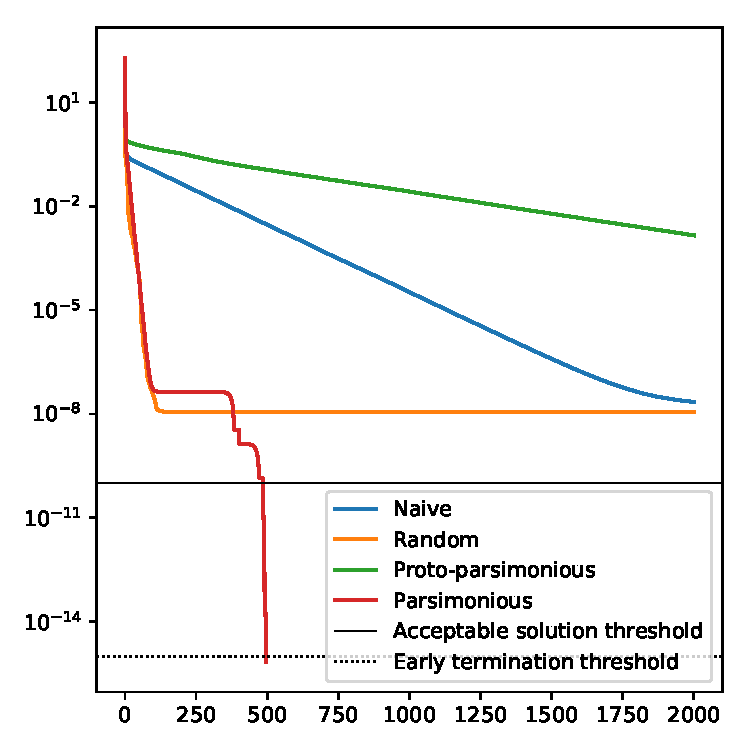
\includegraphics{seed25/figure1-objective}
\caption{\textbf{Objective values.}}
\label{figure:objective}
\end{figure}

\begin{figure}[!ht]
\centering
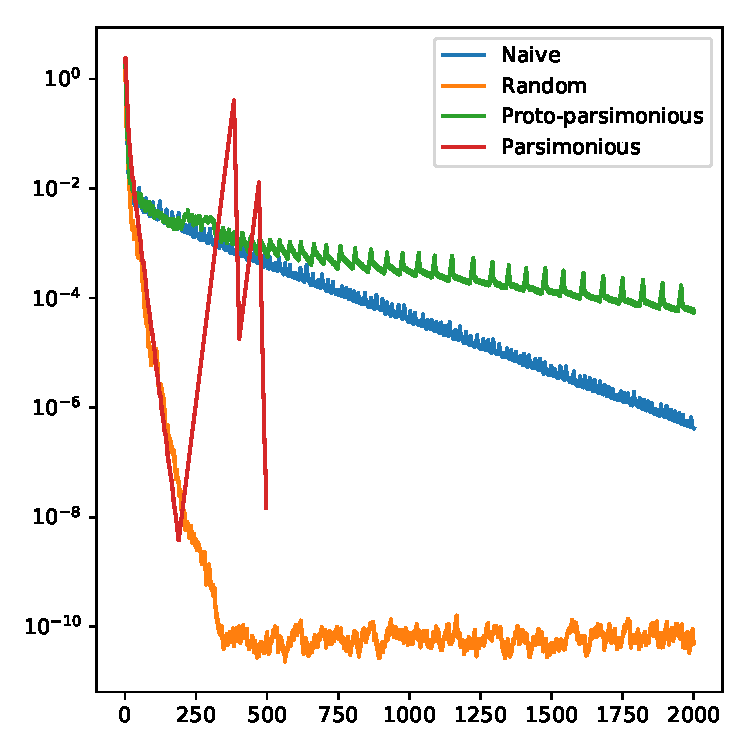
\includegraphics{seed25/figure2-scale}
\caption{\textbf{Size of the `sweep' optimization parameter.}}
\label{figure:sweep}
\end{figure}

\begin{figure}[!ht]
\centering
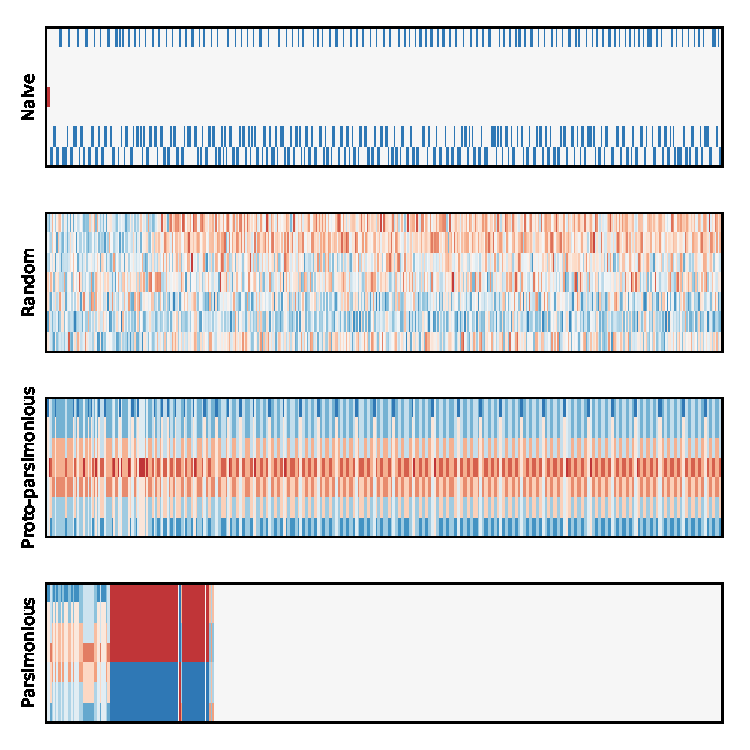
\includegraphics{seed25/figure3-directions}
\caption{\textbf{Selected parameter update directions.}}
\label{figure:directions}
\end{figure}

\begin{figure}[!ht]
\centering
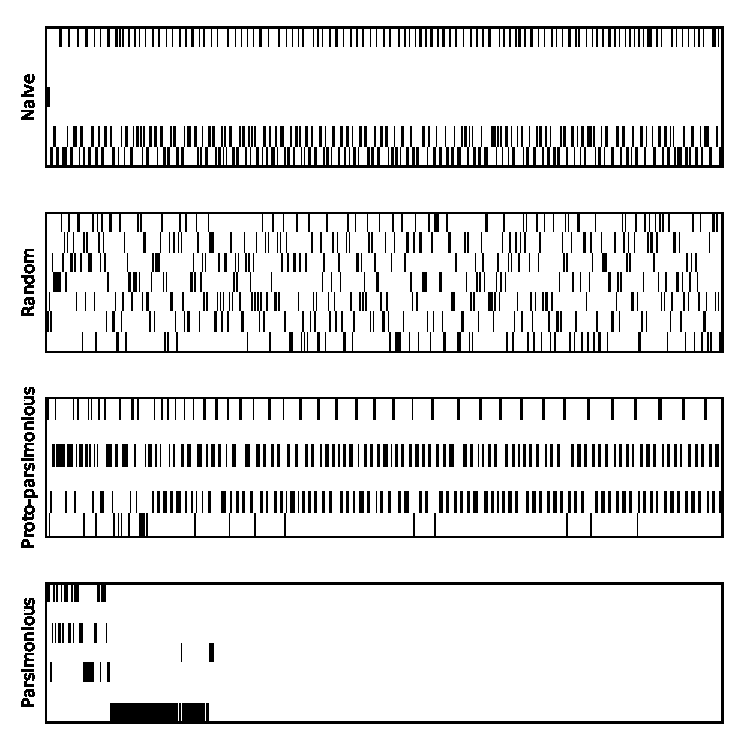
\includegraphics{seed25/figure4-direction_vectors}
\caption{\textbf{Selected search direction vectors.}}
\label{figure:direction-vectors}
\end{figure}

Rather than talking through each figure, I'll instead talk through each approach, building up the problem along the way.  First is the `naive' approach, which we clearly see, in Figure \ref{figure:objective} (blue line), failing to converge to an `acceptable' solution.  Rather it seem to be approaching some local solution.  Early in the optimiation we see a brief period -- maybe tens of iterations -- where the objective value falls dramatically, then a long, slow period where the objective value falls off at some expontentially decreasing rate (evinced by the roughly linear region in the logarithmic space).  A similar trend is observable if we look at how the search scale changes throughout the iterations, in Figure \ref{figure:sweep} (again, blue line).

What exactly is happening when we apply this approach?  Figure \ref{figure:directions}, which shows the direction in which the parameter values change at each step, is suggestive.  (Figure \ref{figure:direction-vectors} shows which search direction vector was selected, which, in this `naive' case, corresponds directly to the model parameters.)  Remarkably it seems that the second, third, fourth and fifth parameters, corresponding to \(c_2\), \(c_3\), \(c_4\), and \(k_A\), are almost never perturbed (if ever).  This suggests that these parameters are very difficult to tune without `breaking' other parts of the problem.  Likewise, the routine alternation between the other three parameters suggests that the direction of greatest local improvement (i.e. the direction oppposite the gradient) is not aligned with the basic model parameters.  Thus it's stuck making marginal gains.

How does the random approach compare?  Initially, as we see in Figure \ref{figure:objective}, much more favorably.  The initial period of rapid decay is much longer and more productive, although it appears to `slam' into the same asymptotic limit as the `naive' approach.  The search scale (Figure \ref{figure:sweep}) falls off dramatically, too.  Figure \ref{figure:direction-vectors} is useless, of course, since the search directions are re-selected each iteration (although we do see that they are clearly random).  As far as the search directions go (Figure \ref{figure:directions}), we see some trends, particularly in the later steps, but nothing too compelling or convincing.

Thus we come to the proto-parsimonious approach.  In this instance, it's actually quite ineffective at solving this problem, seemingly even worse than the prior two approaches.  However, as the random approach demonstrates, rapid collapse of the objective value may be a poor long-term strategy.

The parsimonious approach, on the other hand (which I will note is just the proto-parsimonious approach with one additional search direction!) is far more succesful (Figure \ref{figure:objective}).  It emulates the rapid collapse of the random search approach, although it stops short, plateaus for some time, then starts fall off again -- hitting a few small plateaus until ultimately falling past our early termination point.  Figure \ref{figure:sweep} shows that the search scale is actually ramping up during these plateaus; seemingly, after aggresive exploitation of the local gradient, the problem finds a new, preferable search direction.  Figures \ref{figure:directions} and \ref{figure:direction-vectors} shows that this corresponds exactly to that one additional search direction vector, in which every parameter is modified (in this case, we see that the concentrations are brought down while the kinetic rate constants are raised proportionally).

A few more runs may be illustrative.  In some cases, the last two approaches may closely follow each other for some time.  In other instances none of the approaches converge (though, in my experience, the parsimonious approach will if allowed enough perturbations).  The overall trend of heavy drops followed by plateaus where the seventh search direction is exploited seems consistent.

\section{Discussion}

Most of my analysis is given in the Results, but I'll highlight a couple things.  First, even this simple problem (one which you could readily solve by hand) is hard for an optimization algorithm to solve.  Speculatively this comes down to the structure of the objective space; I believe there are several `plateaus' that a solver must navigate without becoming stuck or simply lost.

Second, despite the fact that it should theoretically search the entire space, random search vectors aren't very effective.  I'm not sure whether this is due to the dimensionality of the problem, or the aggressiveness of a random search, or its inherent aimlessness.

Third, I think it's striking how the proto-parsimonious approach \textit{almost} works, barring that one additional search direction which rescales all of the parameters.  I also think it's incredible how the parsimonious approach seemingly always works while the others practically never work (even though I did, admittedly, contrive this system to demonstrate the value of parsimonious perturbations).

I think the optimization algorithm presented here is obviously not practical, yet contains some useful and promising ideas.  The fact that each iteration scales \(\mathcal{O}\left(n\right)\) with respect to the number of parameters is interesting, as is the adaptive search window approach.

I encourage the reader to play with this system, see its limits.  Try changing the objective or initialization.  Also try other search directions, or combinations of the presented search directions.

\end{document}
